\documentclass[12pt, a4paper]{report}
%\documentclass[11pt, a4paper]{article}

%====================== PACKAGES ======================
\usepackage[french]{babel}

\frenchbsetup{StandardLists=true}
\usepackage{enumitem}
\usepackage{pifont}

\usepackage[utf8x]{inputenc}
%\usepackage[latin1]{inputenc}

%pour gérer les positionnement d'images
\usepackage{float}
\usepackage{amsmath}
\DeclareMathOperator{\dt}{dt}
\usepackage{amsfonts}
\usepackage{graphicx}
%\usepackage{tabularx}
\usepackage[colorinlistoftodos]{todonotes}
\usepackage{url}

%pour les informations sur un document compilé en PDF et les liens externes / internes
\usepackage[pdfborder=0]{hyperref}
\hypersetup{
	colorlinks = true
	}

%pour la mise en page des tableaux
\usepackage{array}
\usepackage{tabularx}
\usepackage{multirow}
\usepackage{multicol}
\setlength{\columnsep}{50pt}

%pour utiliser \floatbarrier
%\usepackage{placeins}
%\usepackage{floatrow}

%espacement entre les lignes
\usepackage{setspace}

%modifier la mise en page de l'abstract
\usepackage{abstract}

%police et mise en page (marges) du document
\usepackage[T1]{fontenc}
\usepackage[top=2cm, bottom=2cm, left=2cm, right=2cm]{geometry}

%Pour les galerie d'images
\usepackage{subfig}

\usepackage{pdfpages}

\usepackage{tikz}
\usetikzlibrary{trees}
\usetikzlibrary{decorations.pathmorphing}
\usetikzlibrary{decorations.markings}
\usetikzlibrary{decorations.pathreplacing,calligraphy}
%\usetikzlibrary{decorations}
\usetikzlibrary{angles, quotes}
\usepackage{verbatim}

\usepackage{appendix}

\usepackage{comment}

\usepackage{xcolor}

%\PreviewEnvironment{tikzpicture}
%\setlength\PreviewBorder{0pt}%

%====================== INFORMATION ET REGLES ======================

%rajouter les numérotation pour les \paragraphe et \subparagraphe
\setcounter{secnumdepth}{4}
\setcounter{tocdepth}{4}

\hypersetup{							% Information sur le document
pdfauthor = {Stephan Runigo},			% Auteurs
pdftitle = {Documentation},			% Titre du document
pdfsubject = {Documentation},		% Sujet
pdfkeywords = {Document},	% Mots-clefs
pdfstartview={FitH}}	% ajuste la page à la largeur de l'écran
%pdfcreator = {MikTeX},% Logiciel qui a crée le document
%pdfproducer = {} % Société avec produit le logiciel

%======================== DEBUT DU DOCUMENT ========================
%
\begin{document}
%
%régler l'espacement entre les lignes
\newcommand{\HRule}{\rule{\linewidth}{0.5mm}}
%
% Titre, résumé, ... %
%
\begin{titlepage}
%
~\\[1cm]

\begin{center}
%\includegraphics[scale=0.5]{./presentation/chambreABulle}
\end{center}

\textsc{\Large }\\[0.5cm]

% Title \\[0.4cm]
\HRule

\begin{center}
{\huge \bfseries  La causalité\\
%titre 2\\[0.4cm]
 }
\end{center}

\HRule \\[1.5cm]

\begin{center}
%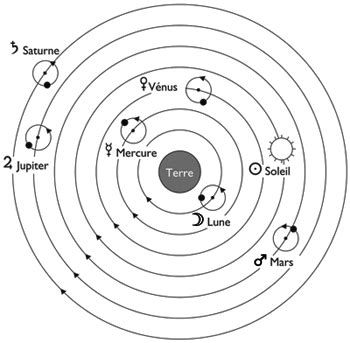
\includegraphics[scale=0.3]{./presentation/ptoleme}
\end{center}

\begin{center}
%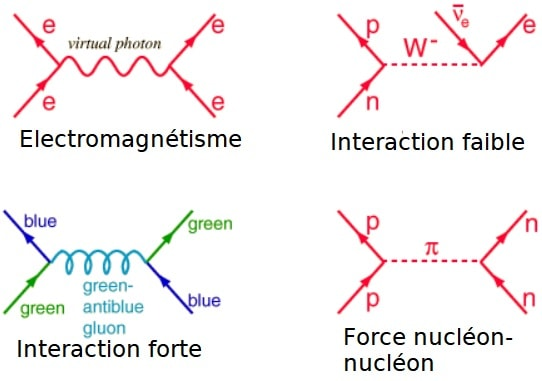
\includegraphics[scale=0.3]{./presentation/diagrammesInteractions}
\end{center}


% Author and supervisor
\begin{minipage}{0.4\textwidth}
\begin{flushleft} \large
%\emph{Auteur:}\\
%Stephan \textsc{Runigo}
\end{flushleft}
\end{minipage}
\begin{minipage}{0.4\textwidth}
\begin{flushright} \large
\emph{Auteur:}\\
Stephan \textsc{Runigo}
\end{flushright}
\end{minipage}

\vfill

% Bottom of the page
{\large \today}

\end{titlepage}

\newpage
\begin{center}
\Large
Résumé
\normalsize
\end{center}
\vspace{3cm}
\begin{itemize}[leftmargin=1cm, label=\ding{32}, itemsep=21pt]
\item {\bf Objet : } Souvenir des questions posés.
\item {\bf Contenu : } Définition, analyse, reflexion.
\item {\bf Public concerné : } Interressé à la question de l'âme.
\end{itemize}

\vspace{3cm}



\vspace{3cm}


%

%
% Table des matières
\tableofcontents
\thispagestyle{empty}
\setcounter{page}{0}
%
%espacement entre les lignes des tableaux
\renewcommand{\arraystretch}{1.5}
%
%====================== INCLUSION DES CHAPITRES ======================
%
~
\thispagestyle{empty}
%recommencer la numérotation des pages à "1"
\setcounter{page}{0}
\newpage
%
\chapter{Forces à distance}
%
Une force modélise une action mécanique : un homme pousse un chariot, le chariot se met en mouvement. L'action est de pousser, c'est une action de contact, son effet est la mise en mouvement. Cette action peut être modélisée par une force : l'homme applique une force sur le chariot.

\begin{center}

\includegraphics[scale=0.6]{./forces/chariotPousse}
\end{center}

Une force est représentée par un vecteur et un point d'application : Le point d'application est le point de contact (A), la force est horizontal, vers la droite et possède une valeur (mesurée en newton).

\begin{center}
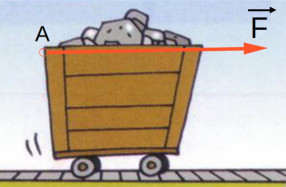
\includegraphics[scale=0.6]{./forces/chariotVecteur}
\end{center}

Nous étudions dans les paragraphes suivants, trois forces à distance (il n'y a pas de contact entre les corps).


%%%%%%%%%%%%%%%%%%%%%
\section{Force gravitationnelle}
%%%%%%%%%%%%%%%%%%%%%
%

L'interaction gravitationnelle est une action à distance entre les corps : les corps ayant une masse s'attirent entre eux, la force gravitationnelle modélise l'interaction gravitationnelle. 

La terre exerce sur la lune une action mécanique dont l'effet est d'{\it incurver} sa trajectoire, sans cette action la lune s'éloignerait de la terre.

\setlength{\unitlength}{1cm}
%
\begin{center}
\mbox{%\fbox{
\begin{picture}(17,3)
\put(2,2){\circle{1.52}}
\put(1.6,0.8){Terre}
\thicklines
\put(2,2){\vector(1,0){2.76}}
\put(4.3,2.3){$\overrightarrow{F}_{L/T}$}
\put(15,2){\circle{0.5}}
\put(14.6,1.2){Lune}
\thicklines
\put(15,2){\vector(-1,0){2.76}}
\put(12,2.3){$\overrightarrow{F}_{T/L}$}
\end{picture}}

$\overrightarrow{F_{L/T}}$ : Force gravitationnelle exercée par la lune sur la terre,

 $\overrightarrow{F_{T/L}}$ : Force gravitationnelle exercée par la terre sur la lune.
\end{center}


%%%%%%%%%%%%%%%%%%%%%%%%%%%%%%%%%%%%%%%%%%%%%%%%%%%%%%%%%%%%%%%%%%%%%%%%%%%%

%

%%%%%%%%%%%%%%%%%%%%%
\section{Champ électrique et potentiel scalaire}
%%%%%%%%%%%%%%%%%%%%%
%
Le champ électrique créé par une particule chargé s'étend dans l'espace à 3 dimensions. Il est possible, afin de simplifier les schéma de se limiter à 2 dimensions.

Le champ électrique créé par une particule chargée est radial et son amplitude décroit avec la distance à la particule.

\begin{center}
\tikzstyle{fleche}=[->,line width=1pt]
\begin{tikzpicture}
  \begin{scope}[xshift=0 cm,yshift=0 cm, scale = 1.6]%
\foreach \t in {60,120, ...,360}
\draw [fleche] (\t:1) -- (\t:2.8);
\foreach \t in {30,90, ...,360}
\draw [fleche] (\t:2) -- (\t:2.45);
\foreach \t in {15,45,-15,-45}
\draw [fleche] (\t:3) -- (\t:3.2);
\foreach \t in {15,45,-15,-45}
\draw [fleche] (\t+180:3) -- (\t+180:3.2);
\draw [fill=red] (0,0) circle(0.1) node [above right] {$Q_1$};
  \end{scope}
\end{tikzpicture}
\end{center}


Comme le champ de pente dérive d'un champ scalaire (le champ d'altitude), le champs electrique dérive d'un champ scalaire. On l'appelle le potentiel électrique. On représente ci-dessous les lignes de même potentiel (équi-potentiel) du potentiel électrique créé par une particule chargée.

\begin{center}
\begin{tikzpicture}
  \begin{scope}[xshift=0 cm,yshift=0 cm, scale = 1]%
\foreach \t in {1,2, ...,30}
\draw [line width=1pt] (0,0) circle (5/\t) ;

\draw [fill=red] (0,0) circle(0.2) node [above right,text=white] {$Q_1$};
  \end{scope}
\end{tikzpicture}
\end{center}

En 3 dimensions, les points de même potentiel sont des surfaces. Les surfaces équi-potentiel du potentiel créé par une particule chargée sont des sphères.

%%%%%%%%%%%%%%%%%%%%%%%%%%%%%%%%%%%%%%%%%%%%%%%%%%%%%%%%%%%%%%%%%%%%%%%%%%%%

%

%%%%%%%%%%%%%%%%%%%%%
\section{Force magnétique}
%%%%%%%%%%%%%%%%%%%%%
%

La force magnétique est la force qui s'exerce entre les \textbf{\textit {aimants}}.
Les aimants sont des matériaux possédant des propriétés magnétiques.
Certain métaux peuvent être aimantés par la proximité d'un aimant.

\subsection{Pôles magnétiques}

Un aimants est toujours {\it orienté}, il possède un pôle dit \textbf{\textit {nord}} et un pôle
dit \textbf{\textit {sud}}.


\subsection{Action magnétique}

La force magnétique entre deux aimants, est attractive et répulsive, elle exerce un {\it couple} :
entre deux aimants, les pôles opposés s'attirent, les pôles identiques se repoussent. 

Ci-dessous, deux aimants sont schématisés, les pôles nord en rouge et les pôles sud en bleu. On ne représente que les forces que l'aimant 2 exerce sur l'aimant 1.

\begin{center}
\begin{tikzpicture}[scale=1]
\fill [blue] (0,0) rectangle (0.3,1.5);
\fill [red] (0,1.5) rectangle (0.3,3);
\begin{scope}[rotate=30,yshift=-4.2cm]%
\fill [red] (8,0) rectangle (8.3,1.5);
\fill [blue] (8,1.5) rectangle (8.3,3);
\end{scope}
\thicklines
\put(0.15,0.15){\vector(1,0){1.76}}
\put(2,0.3){$\overrightarrow{F}_{N_2/S_1}$}

\put(0.15,2.85){\vector(1,0){2.26}}
\put(2.6,3){$\overrightarrow{F}_{S_2/N_1}$}

\draw [thick] [->] ((0.15,(0.15) --++(-1.5,-0.7) node [left] {$\overrightarrow{F}_{N_2/N_1}$};

\draw [thick] [->] ((0.15,(2.85) --++(-0.8,0.3) node [left] {$\overrightarrow{F}_{S_2/S_1}$};

%\put(0.15,0.15){\vector(-1,-1){0.5}}
%\put(4.3,2.3){$\overrightarrow{F}_{L/T}$}
\end{tikzpicture}
\end{center}
%%%%%%%%%%%%%%%%%%%%%%%%%%%%%%%%%%%%%%%%%%%%%%%%%%%%%%%%%%%%%%%%%%%%%%%%%%%%

%
%\input{.//.tex}

%

%%%%%%%%%%%%%%%%%%%%%
\section{Champs quantiques}
%%%%%%%%%%%%%%%%%%%%%
%
Une particule élémentaire est décrite par une fonction d'onde. Un ensemble de particules élémentaires identiques sont décrites par la superposition, la somme, des fonctions d'ondes individuelles. Ce champ total, pour un type de particule est à même de décrire l'ensemble de ces particules.

Ainsi, l'ensemble des électrons est décrit par le champ électron, l'ensemble des photons est décrit par le champ photon. Ces deux champs sont présent dans l'espace temps, la détection d'un photon ou d'un électron est due à un échange élémentaire d'énergie entre ces deux champs.

Lorsqu'un photon se matérialise en une paire électron-positron : un transfert d'énergie s'oppère du champ photon vers le champ électron. Lorsqu'un électron rencontre un positron, ils s'anihilent donnant un photon :  un transfert d'énergie s'oppère du champ électron vers le champ photon.

Une particule élémentaire peut alors être considérée comme l'évènement : transfert d'énergie entre deux champs quantique, la matière classique ne serait donc que la manifestation de ces évenements.

Les évènement de transfert d'énergie entre deux champs quantique caractérise le \textsf{\textit {couplage}} entre les champs.

L'existence (ou la détection) de la force électrique entre un électron et un proton serait la signature du couplage entre le champ électron et le champ photon d'une part et du couplage entre le champ proton et le champ photon. Le champ photon est le médiateur de la force électrique entre les particules chargées.
%%%%%%%%%%%%%%%%%%%%%%%%%%%%%%%%%%%%%%%%%%%%%%%%%%%%%%%%%%%%%%%%%%%%%%%%

%
\chapter{Champs et potentiel}
%
%

%%%%%%%%%%%%%%%%%%%%%
\section{Pente et altitude}
%%%%%%%%%%%%%%%%%%%%%
%
Le paysage ci-dessous est constitué de deux collines. La colline de gauche possède un coté très pentu. La colline de droite est moins haute. Un village se trouve à proximité du col.

\vfill
\begin{center}
\includegraphics[scale=0.7]{./potentiel/collines}
\end{center}

\vfill
Comment représenter ce paysage, qui est un relief en 3 dimensions, sur une carte en 2 dimensions ?

Nous allons voir deux façons de représenter ce relief : 

\vfill
\begin{minipage}[c]{.45\linewidth}
{\bf Les lignes de niveau} : c'est un champ scalaire (que l'on apellera champ d'altitude), donnant l'altitude du point considéré.

{\bf Les vecteurs "pente"} : c'est un champ vectoriel (que l'on apellera champ de pente), donnant la direction et l'importance de la pente (les vecteurs rouges ci-contre en donnent quelques exemples).
\end{minipage}
\hfill
\begin{minipage}[c]{.45\linewidth}
\begin{center}
\includegraphics[scale=0.4]{./potentiel/altitude}
\end{center}
\end{minipage}

\vfill
\newpage
%Sur une carte topographique, les lignes de niveaux sont utilisées. Alors que la surface de la terre est en 3 dimensions, 
%Une carte routière en 2 dimensions montre une vue de dessus suffisante. Sur une carte topographique, l'altitude est représenté en plus de la vue de dessus grâce aux lignes de niveau.

\subsection{"Champ d'altitude"}

Sur une carte topographique, le relief est représenté par des lignes de niveau, des lignes de même altitude.

Sur le schéma suivant, le paysage précédent est représenté vu de dessus. Son relief y est représenté à l'aide des lignes de niveau.

Les points d'altitudes 300 m, 350 m , et 400 m se trouve sur les lignes en gras en gras, les lignes en trait fin indiquent les points d'altitudes intermédiaires multiple de 10 (310 m, 320 m, 330 m, etc...)

%\vfill
\begin{center}
\includegraphics[scale=0.6]{./potentiel/potentiel}
\end{center}

%\vfill

En chaque point de la carte, on peut lire l'altitude en s'aidant des lignes de niveau (Le village se trouve à une altitude d'environ 295 m). Les lignes de niveau représentent donc un champ (le "champ d'altitude") dans un espace a 2 dimension (la carte), il s'agit d'un champ scalaire (l'altitude est un nombre).

Ces lignes sont plus proches les unes des autres lorsque la pente est plus forte.

%Nous allons voir qu'il existe une autre représentation du relief : le "champs de pente".

\vfill
\newpage
\subsection{"Champ de pente"}

Le "champs de pente" est un champ vectoriel, en chaque point de la carte, on représente la pente par un vecteur dirigé dans le sens de la pente et dont la longueur est proportionnel à la pente (d'autant plus grande que la pente est grande).

Le schéma ci-dessous représente le "vecteur pente" en quelques points de la carte. On constate que celui-ci est "grand" dans la zone pentu de la colline de gauche.

%\vfill
\begin{center}
\includegraphics[scale=0.7]{./potentiel/vecteur}
\end{center}

%\vfill
On remarque alors que le vecteur "champs de pente" est perpendiculaire au ligne de niveau du champs "d'altitude".

\vfill
\newpage
%%%%%%%%%%%%%%%%%%%%%%%%%%%%%%%%%%%%%%%%%%%%%%%%%%%%%%%%%%%%%%%%%%%%%%%%%%%%

%

%%%%%%%%%%%%%%%%%%%%%
\section{Champ électrique et potentiel scalaire}
%%%%%%%%%%%%%%%%%%%%%
%
Le champ électrique créé par une particule chargé s'étend dans l'espace à 3 dimensions. Il est possible, afin de simplifier les schéma de se limiter à 2 dimensions.

Le champ électrique créé par une particule chargée est radial et son amplitude décroit avec la distance à la particule.

\begin{center}
\tikzstyle{fleche}=[->,line width=1pt]
\begin{tikzpicture}
  \begin{scope}[xshift=0 cm,yshift=0 cm, scale = 1.6]%
\foreach \t in {60,120, ...,360}
\draw [fleche] (\t:1) -- (\t:2.8);
\foreach \t in {30,90, ...,360}
\draw [fleche] (\t:2) -- (\t:2.45);
\foreach \t in {15,45,-15,-45}
\draw [fleche] (\t:3) -- (\t:3.2);
\foreach \t in {15,45,-15,-45}
\draw [fleche] (\t+180:3) -- (\t+180:3.2);
\draw [fill=red] (0,0) circle(0.1) node [above right] {$Q_1$};
  \end{scope}
\end{tikzpicture}
\end{center}


Comme le champ de pente dérive d'un champ scalaire (le champ d'altitude), le champs electrique dérive d'un champ scalaire. On l'appelle le potentiel électrique. On représente ci-dessous les lignes de même potentiel (équi-potentiel) du potentiel électrique créé par une particule chargée.

\begin{center}
\begin{tikzpicture}
  \begin{scope}[xshift=0 cm,yshift=0 cm, scale = 1]%
\foreach \t in {1,2, ...,30}
\draw [line width=1pt] (0,0) circle (5/\t) ;

\draw [fill=red] (0,0) circle(0.2) node [above right,text=white] {$Q_1$};
  \end{scope}
\end{tikzpicture}
\end{center}

En 3 dimensions, les points de même potentiel sont des surfaces. Les surfaces équi-potentiel du potentiel créé par une particule chargée sont des sphères.

%%%%%%%%%%%%%%%%%%%%%%%%%%%%%%%%%%%%%%%%%%%%%%%%%%%%%%%%%%%%%%%%%%%%%%%%%%%%

%

%%%%%%%%%%%%%%%%%%%%%
\section{Force magnétique}
%%%%%%%%%%%%%%%%%%%%%
%

La force magnétique est la force qui s'exerce entre les \textbf{\textit {aimants}}.
Les aimants sont des matériaux possédant des propriétés magnétiques.
Certain métaux peuvent être aimantés par la proximité d'un aimant.

\subsection{Pôles magnétiques}

Un aimants est toujours {\it orienté}, il possède un pôle dit \textbf{\textit {nord}} et un pôle
dit \textbf{\textit {sud}}.


\subsection{Action magnétique}

La force magnétique entre deux aimants, est attractive et répulsive, elle exerce un {\it couple} :
entre deux aimants, les pôles opposés s'attirent, les pôles identiques se repoussent. 

Ci-dessous, deux aimants sont schématisés, les pôles nord en rouge et les pôles sud en bleu. On ne représente que les forces que l'aimant 2 exerce sur l'aimant 1.

\begin{center}
\begin{tikzpicture}[scale=1]
\fill [blue] (0,0) rectangle (0.3,1.5);
\fill [red] (0,1.5) rectangle (0.3,3);
\begin{scope}[rotate=30,yshift=-4.2cm]%
\fill [red] (8,0) rectangle (8.3,1.5);
\fill [blue] (8,1.5) rectangle (8.3,3);
\end{scope}
\thicklines
\put(0.15,0.15){\vector(1,0){1.76}}
\put(2,0.3){$\overrightarrow{F}_{N_2/S_1}$}

\put(0.15,2.85){\vector(1,0){2.26}}
\put(2.6,3){$\overrightarrow{F}_{S_2/N_1}$}

\draw [thick] [->] ((0.15,(0.15) --++(-1.5,-0.7) node [left] {$\overrightarrow{F}_{N_2/N_1}$};

\draw [thick] [->] ((0.15,(2.85) --++(-0.8,0.3) node [left] {$\overrightarrow{F}_{S_2/S_1}$};

%\put(0.15,0.15){\vector(-1,-1){0.5}}
%\put(4.3,2.3){$\overrightarrow{F}_{L/T}$}
\end{tikzpicture}
\end{center}
%%%%%%%%%%%%%%%%%%%%%%%%%%%%%%%%%%%%%%%%%%%%%%%%%%%%%%%%%%%%%%%%%%%%%%%%%%%%

%
%\input{./potentiel/.tex}
%

%
%
\begin{appendix}
%

%%%%%%%%%%%%%%%%%%%%%
\chapter{Glossaire}
%%%%%%%%%%%%%%%%%%%%%

\begin{itemize}[leftmargin=1cm, label=\ding{32}, itemsep=2pt]
\item {\bf application} : en mathématique, synonyme de fonction.
\item {\bf } :
\item {\bf } :
\item {\bf quanton} : particule élémentaire satisfaisant à l'équation de schrödinger.
\item {\bf } :
\item {\bf } :
\item {\bf } :
\end{itemize}


%%%%%%%%%%%%%%%%%%%%%%%%%%%%%%%%%%%%%%%%%%%%%%%%%%%%%%%%%%%%%%%%%%%%%%%%%%%%%%%%%%%%%

%

%%%%%%%%%%%%%%%%%%%%%
\chapter{Espace vectoriel}
%%%%%%%%%%%%%%%%%%%%%

%%%%%%%%%%%%%%%%%%%%%%%%%
\section{Ensemble et application}
%%%%%%%%%%%%%%%%%%%%%%%%%
%$\mathcal{}$
Un ensemble est une collection d'objets. Ces objets sont appelés éléments (a) de l'ensemble ($\mathcal{A}$) :
\[
 a \in \mathcal{A}
\]


Une application ($f$) met en relation chaque élément ($a$) d'un ensemble ($\mathcal{A}$, dit de départ) avec un élément ($b$) d'un autre ensemble ($\mathcal{B}$, dit d'arrivé) :
\begin{align*}
f :\ \ \ \ \ \ \ \ \ \mathcal{A} \ \  & \rightarrow \ \ \ \mathcal{B} \\
a \ \ & \mapsto \ \ b = f(a)
\end{align*}

Une loi de composition est une application qui associe deux éléments (éventuellement du même ensemble) à un troisième élément. 
\begin{align*}
f :\ \ \ \ \ \ \ \ \ \mathcal{A} \times \mathcal{B} \ \  & \rightarrow \ \ \ \mathcal{C} \\
(a,b) \ \ & \mapsto \ \ c = f(a,b)
\end{align*}

Une loi de composition est dite interne si $\mathcal{A} = \mathcal{B} = \mathcal{C}$, externe sinon.



%%%%%%%%%%%%%%%%%%%%%%%%%
\section{Espace vectoriel}
%%%%%%%%%%%%%%%%%%%%%%%%%
%
Un espace vectoriel est un ensemble (ses éléments sont appelés vecteur), possédant une loi de composition interne (la somme de deux vecteurs d'un espace vectoriel appartient à cet espace) et une loi de composition externe (la multiplication par un scalaire d'un vecteur d'un espace vectoriel appartient à cet espace).


%%%%%%%%%%%%%%%%%%%%%%%%%%%%%%%%%%%%%%%%%%%%%%%%%%%%%%%%%%%%%%%%%%%%%%%%%%%%%%%%%%%%%

%

%%%%%%%%%%%%%%%%%%%%%
\chapter{Transformation de fourier}
%%%%%%%%%%%%%%%%%%%%%

%%%%%%%%%%%%%%%%%%%%%%%%%
\section{Série de fourier}
%%%%%%%%%%%%%%%%%%%%%%%%%
%
Une fonction périodique (de période $T$) est égale à une somme discrète de sinusoïde :
\[
f_T(x)=a_0 + \sum_{n=1}^\infty \left( a_n \cos \frac{2 n \pi x}{T} + b_n \sin \frac{2 n \pi x}{T} \right)
\]
$a_n$ et $b_n$ sont les coefficient de fourier de $f_T(x)$.

%%%%%%%%%%%%%%%%%%%%%%%%%
\section{Transformé de fourier}
%%%%%%%%%%%%%%%%%%%%%%%%%
%
Une fonction quelconque est égale à une somme continue de sinusoïde :
\[
f(x) = \int_{-\infty}^\infty e^{2 i \pi \nu x}\widehat{f}(\nu) d\nu
\]
$\widehat{f}(\nu)$ est la transformé de fourier de $f(x)$.

%%%%%%%%%%%%%%%%%%%%%%%%%%%%%%%%%%%%%%%%%%%%%%%%%%%%%%%%%%%%%%%%%%%%%%%%%%%%%%%%%%%%%

%
%\newpage
%
\end{appendix}
%

%
%====================== INCLUSION DE LA BIBLIOGRAPHIE ======================
%
%récupérer les citation avec "/footnotemark" : 
\nocite{*}
%
% choix du style de la biblio
\bibliographystyle{plain}
%
% inclusion de la biblio
\cleardoublepage
\addcontentsline{toc}{chapter}{Bibliographie}
\bibliography{bibliographie.bib}
%
%====================== FIN DU DOCUMENT ======================
%
\end{document}
%%%%%%%%%%%%%%%%%%%%%%%%%%%%%%%%%%%%%%%%%%%%%%%%%%%%%%%%%%%%%%%%%%%%%%%%%%%%%%%%%
